\documentclass[tikz,border=6pt]{standalone}
\usepackage{xcolor}
\usetikzlibrary{arrows.meta,positioning}

\definecolor{axisgray}{HTML}{333333}
\definecolor{lineblue}{HTML}{4A90D9}
\definecolor{bandgreen}{HTML}{3C763D}
\definecolor{warnred}{HTML}{E74C3C}

\begin{document}
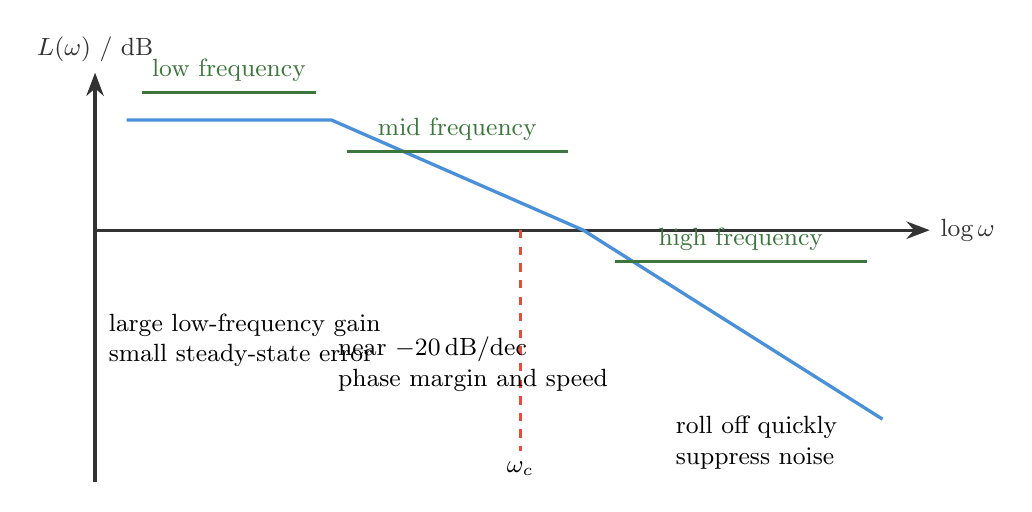
\begin{tikzpicture}[>=Stealth, line width=1.2pt, font=\small]
  \draw[axisgray, ->] (0,0) -- (10.6,0) node[right] {$\log \omega$};
  \draw[axisgray, ->] (0,-3.2) -- (0,2.0) node[above] {$L(\omega)$ / dB};
  \draw[lineblue] (0.4,1.4) -- (3.0,1.4) -- (6.2,0.0) -- (10.0,-2.4);
  \draw[bandgreen] (0.6,1.75) -- (2.8,1.75);
  \node[bandgreen, above] at (1.7,1.75) {low frequency};
  \draw[bandgreen] (3.2,1.0) -- (6.0,1.0);
  \node[bandgreen, above] at (4.6,1.0) {mid frequency};
  \draw[bandgreen] (6.6,-0.4) -- (9.8,-0.4);
  \node[bandgreen, above] at (8.2,-0.4) {high frequency};
  \draw[warnred, dashed] (5.4,0) -- (5.4,-2.8);
  \node[below] at (5.4,-2.8) {$\omega_c$};
  \node[align=left] at (1.9,-1.4) {large low-frequency gain\\small steady-state error};
  \node[align=left] at (4.8,-1.7) {near $-20\,\mathrm{dB/dec}$\\phase margin and speed};
  \node[align=left] at (8.4,-2.7) {roll off quickly\\suppress noise};
\end{tikzpicture}
\end{document}
